\documentclass[a4paper,12pt,twoside]{article}
\usepackage[english]{babel}
\usepackage[utf8]{inputenc}
 \usepackage{placeins}
\usepackage{graphicx}
\usepackage{amsmath}
\usepackage{rotating}
\usepackage{float}
\usepackage{placeins}
\usepackage{graphics}
\usepackage{fixltx2e}
\usepackage[square, colon, super, sort&compress]{natbib}



\graphicspath{ {/home/gerick/Documents/Figures/} }
\pagestyle{headings}
 
\begin{document}
\title{Schnagel Lab Rotation - Modeling of Early Fly Olfaction\\
  \large \textit{Always be faking data}}
\author{Gerick Lee}
\date{}
\maketitle
\section{Introduction}

Partially inspired by the work of Bell, Sawtell, and their colleagues\cite{Bell1993, Bell2000,  Bell1981, Kennedy2014}, we sought to model the early olfactory stages of  \textit{Drosophila.}  We hypothesized that the onset transient seen in Olfactory Receptor Neurons (ORNs) might be removed by the Local Neurons (LNs) in a manner similar to that seen in the weakly electric fish.  If a plastic system could adjust itself to faithfully represent an input stimulus, it would provide an explanation for the emergence of such behavior \textit{in vivo}; an explanation that doesn't depend on a genetic or other pre-programmed factor.

To model this, we used a model of ORNs similar to that in \citet{Nagel2011}.  Both linear (convolutional) models and dynamical firing rate models were created, and were fed into a delay-line LN model, where increases in the odor strength (not the ORNs) would generate a single firing rate increase after a fixed delay.  These firing rates were then fed into a model of the Projection Neurons (PNs), which used a simple anti-Hebbian learning rule to adjust the weights of the inhibitory neurons.  Further circuit properties are described in \citet{Wilson2013}.

\section{Groundwork}
As a first step, we needed to generate reliable gaussian filters (the linear ORN models were generated using either a difference-of-gaussians or gaussian-by-line multiplication).  Figure \ref{fig:filt} shows a test signal (\textit{\textbf{A}}) and the frequency representation of that signal, with an overlapping gaussian filter (\textit{\textbf{B}}).  The filter has a Full-Width-at-Half-Max (FWHM) of 2 Hz, which can be seen in the figure.  

\begin{figure}
\centering

\caption{\textbf{A:} Example signal with non-zero components at the DC, 2Hz, and 3Hz.  \textbf{B:} Fourier Transform of signal (blue), as well as (amplitude-adjusted) filter (red) with FWHM = 2 Hz.\newline}
\hspace*{-3.25cm}
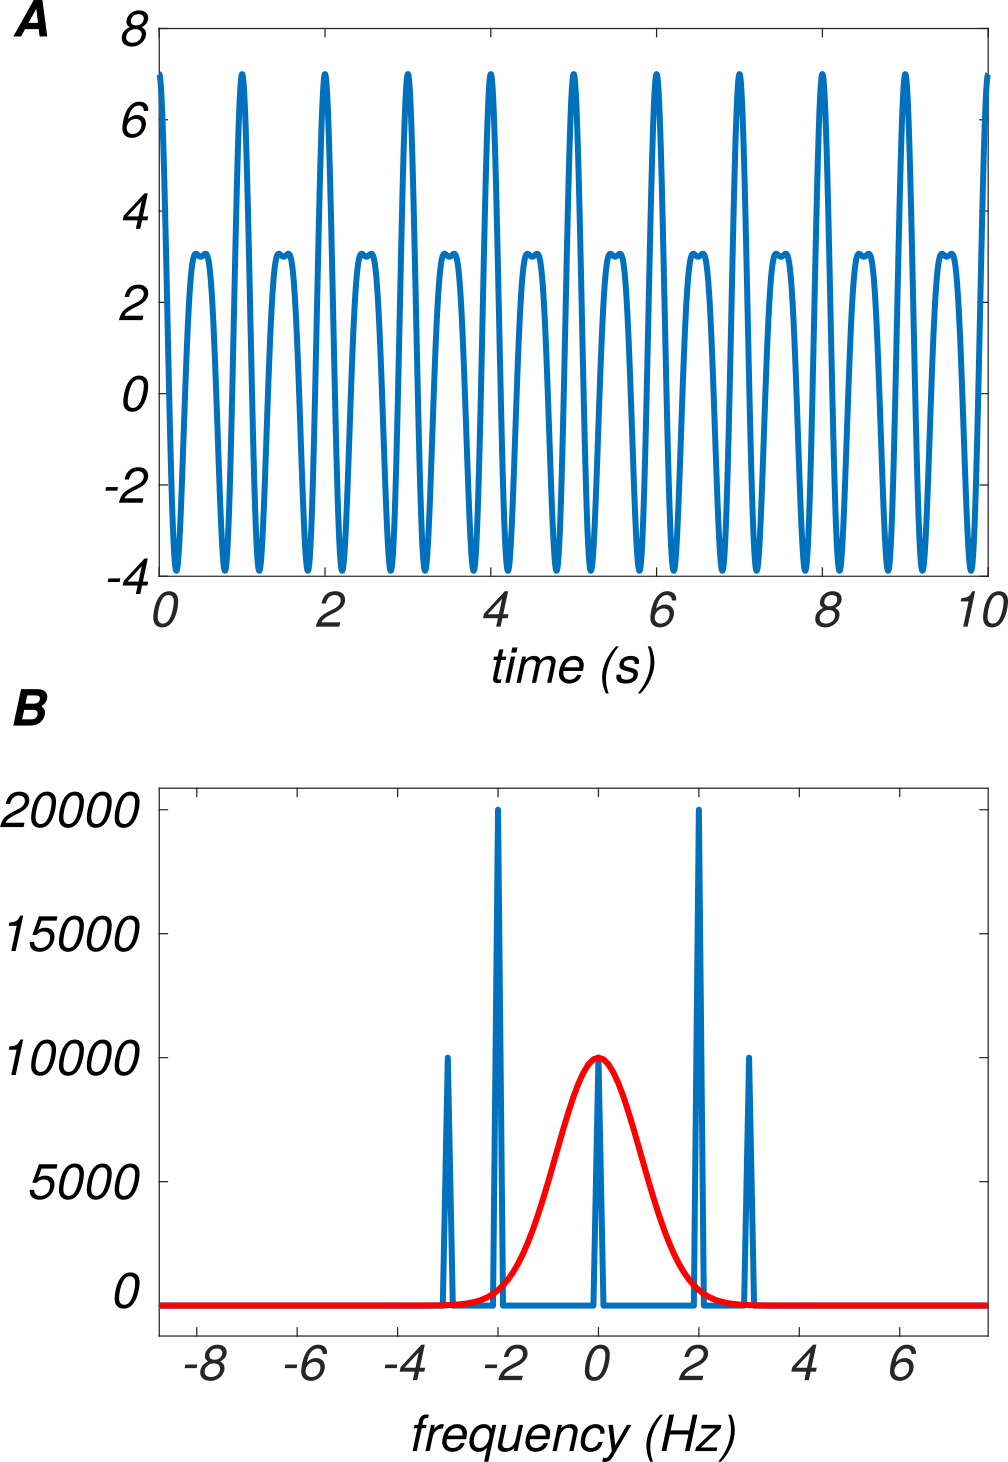
\includegraphics[scale=0.7]{2016-06-16FilterExample.png}
\label{fig:filt}
\end{figure}

\subsection{Odor}
As an input for my model system, we generated a simulated odor as a zero vector with the length of the desired simulation (with a simulated sample rate of $1000$ Hz).  we then generated simulated step odor presentations by setting consecutive windows to a fixed value (in this case $0.5$), for a period corresponding to a desired presentation length (usually $1$ to $1.5$ seconds, or $1000-1500$ samples).  An example section of an odor stimulus is shown as Figure \ref{fig:odor}.

\begin{figure}
\centering
\caption{\textbf{Example odor pulse} \newline}
\hspace*{-1cm}
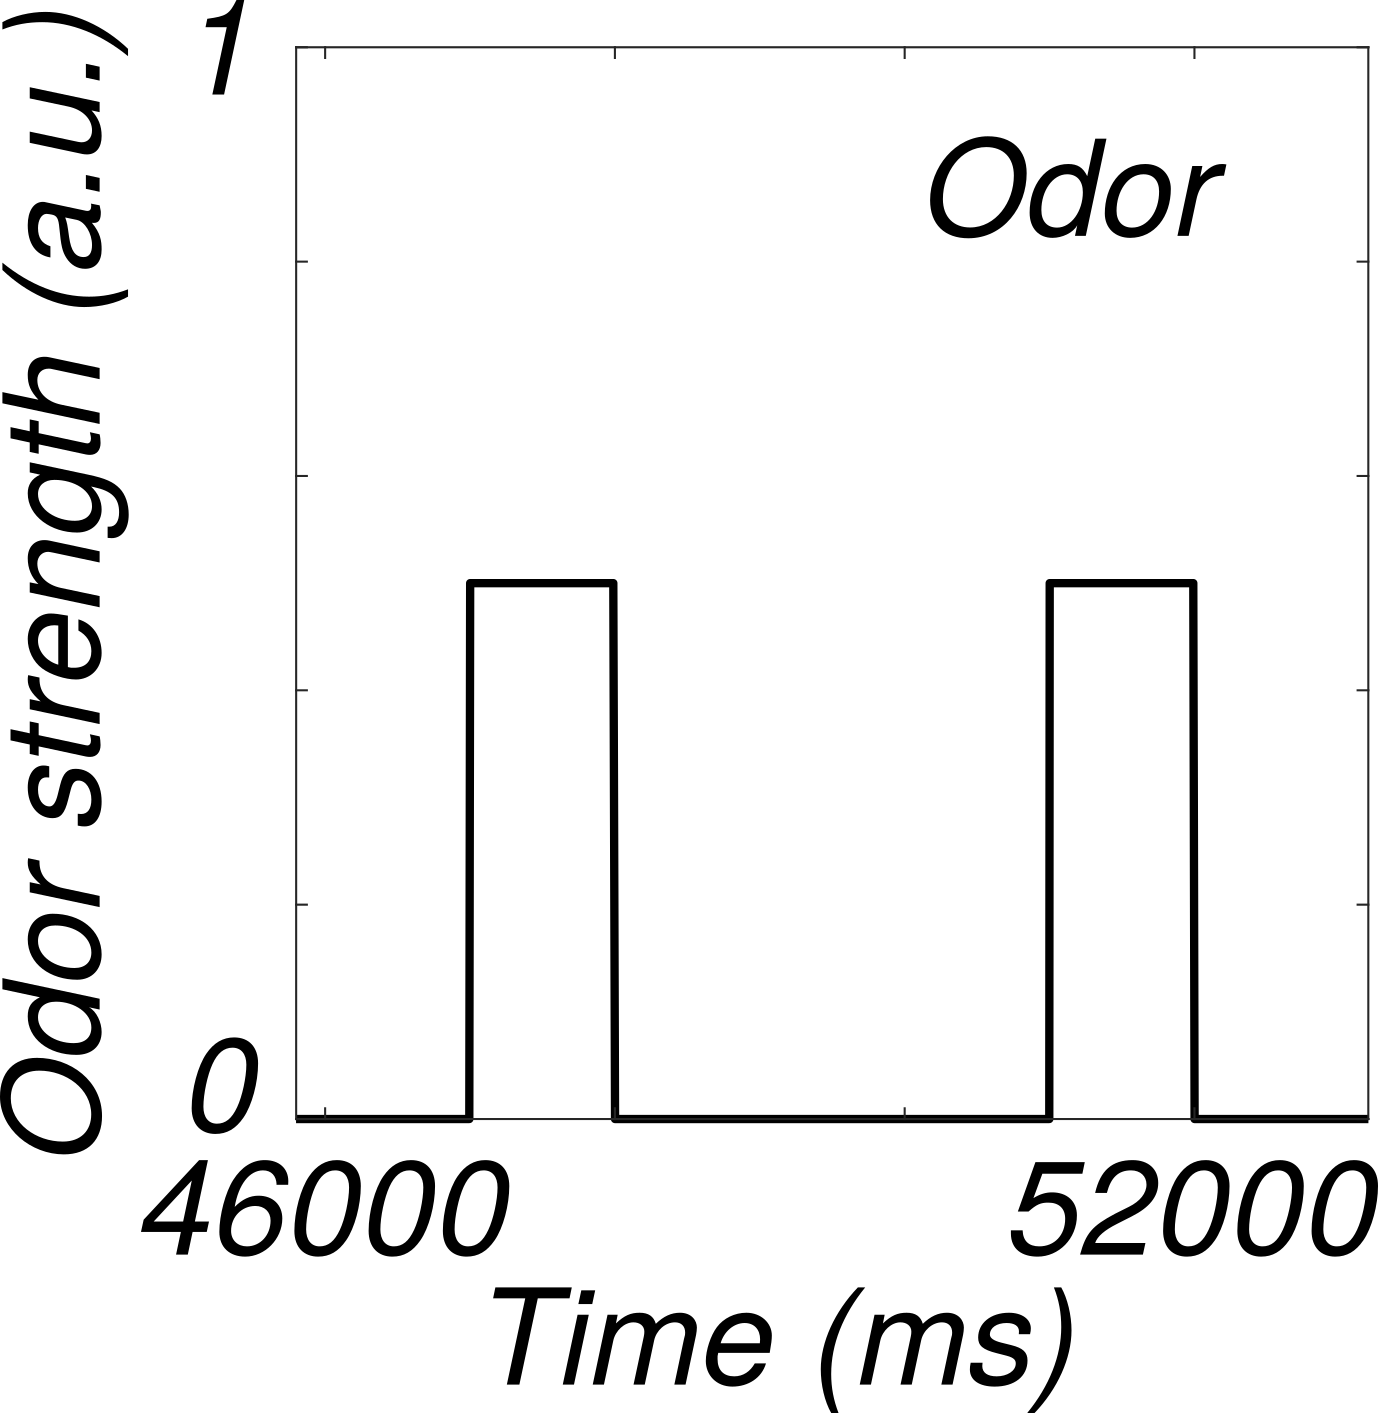
\includegraphics[scale=0.7]{2016-08-26_Example_Odor.png}
\label{fig:odor}
\end{figure}


%\chapter{Methods}
\section{ORN Modelling}
For our investigation of PN responses, we first needed a model of ORNs.  We began with a linear filter model before moving to a dynamical model, inspired by success of the model in \citet{Nagel2011}.
\subsection{Linear Filter Models}
\subsubsection{Difference-of-Gaussian Model}
To model ORNs, we first used a linear filter model using both Difference-of-Gaussians (DoG) and line-gaussian multiplication as my filters in the frequency domain.  Our first attempt used a DoG filter with five parameters (governing the width of each gaussian, as well as their offset from the signal, and each other). Figure \ref{fig:orn1} shows an example curve.  Note that it is possible to rectify the response at zero, so as to better capture the asymmetries observed \textit{in vivo.}

\begin{figure}
\centering
\caption{\textbf{Difference-of-Gaussian based linear filter model} Odor pulse (in arbitrary units) is shown in blue.}
\hspace*{-1.25cm}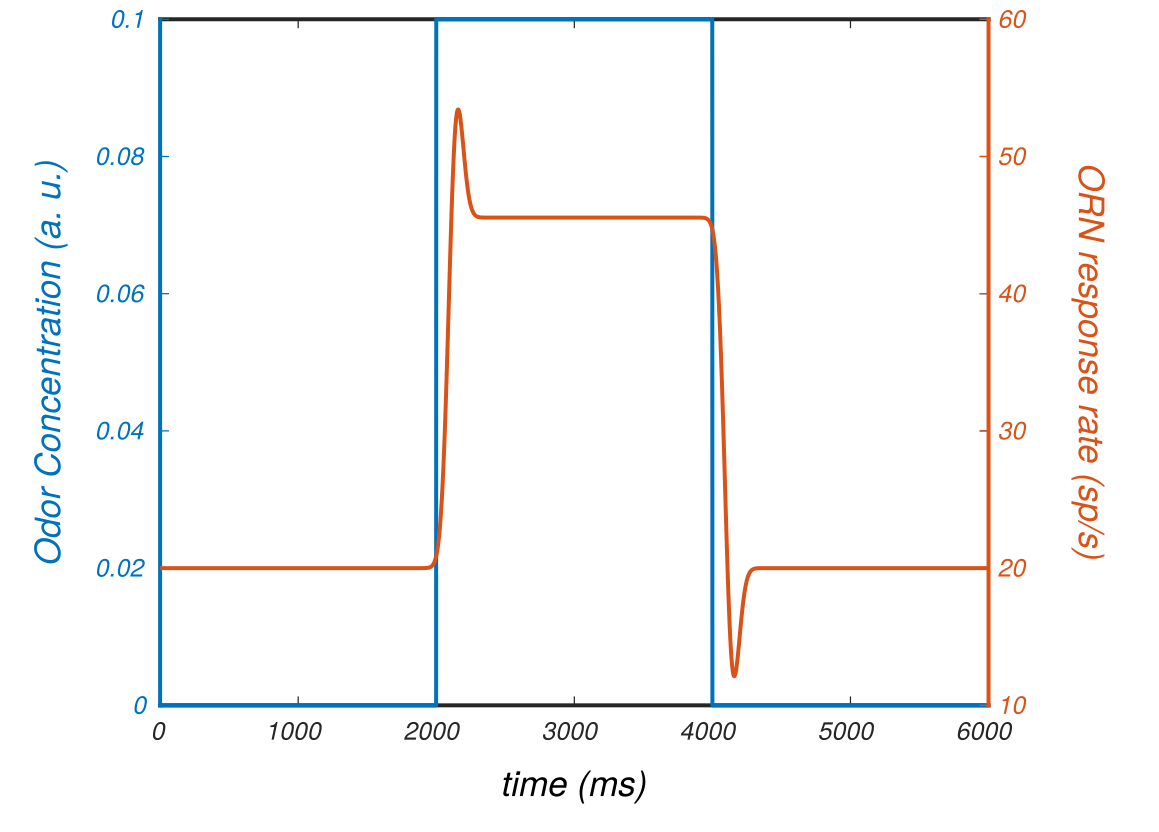
\includegraphics[scale=1]{2016-06-17ModelORNresponse.png}
\label{fig:orn1}
\end{figure}
\subsubsection{Gaussian-Line Model}
To reduce the number of free parameters, we replaced the DoG filter with one multiplying a gaussian filter with a line.  This model was also rectified at zero, to avoid negative firing rates (and return more realistic ORN responses).  Three example responses (two onset, one offset - all of which were generated using the same function [off and onset are determined by the same parameters]) are shown in Figure \ref{fig:orn2}.  



\begin{figure}
\centering
\caption{\textbf{Variability in ORN firing rates: gaussian-by-line model.}  Odor strength (in black, at bottom) is in arbitrary units. \newline}
\hspace*{1.25cm}
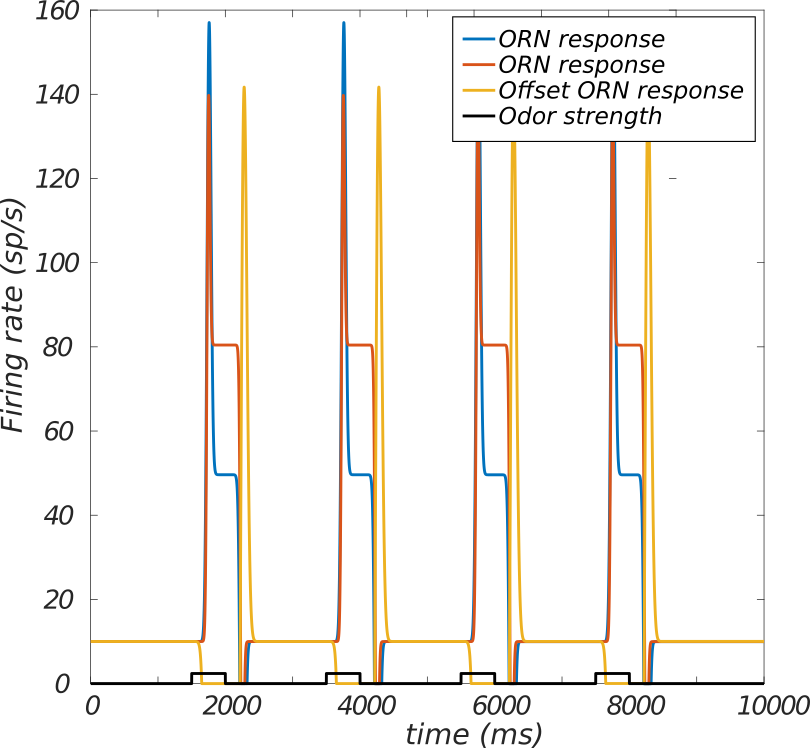
\includegraphics[scale=1.2]{2016-08-05_gauss_line_linear_model.png}
\label{fig:orn2}
\end{figure}

\subsection{Dynamic Model}
For greater accuracy, we switched to a dynamic model of receptor function.  This model was governed by the following:
\begin{equation}
\frac{dR^*}{dt} = k_{on}[O] - (k_{on}[O] + k_{off})R^*,
\end{equation}
where $R^*$ is the proportion of bound receptor (between 0 and 1), $[O]$ is the odor concentration, and there are two rate constants $k.$  This curve could be multiplied by an arbitrary scalar to better reflect real-world firing rates.

In this model (Figure \ref{fig:orn3}) activation alone varies with concentration (as in \cite{Nagel2011}).  This model also saturates with increasing concentration (as a result of the limited range of $R^*$).

\begin{figure}
\centering
\caption{\textbf{ORN firing rates: Basic dynamic model.}  Odor strength (in black, at bottom) is in arbitrary units, though relative magnitudes are preserved.\newline}
\hspace*{-1cm}
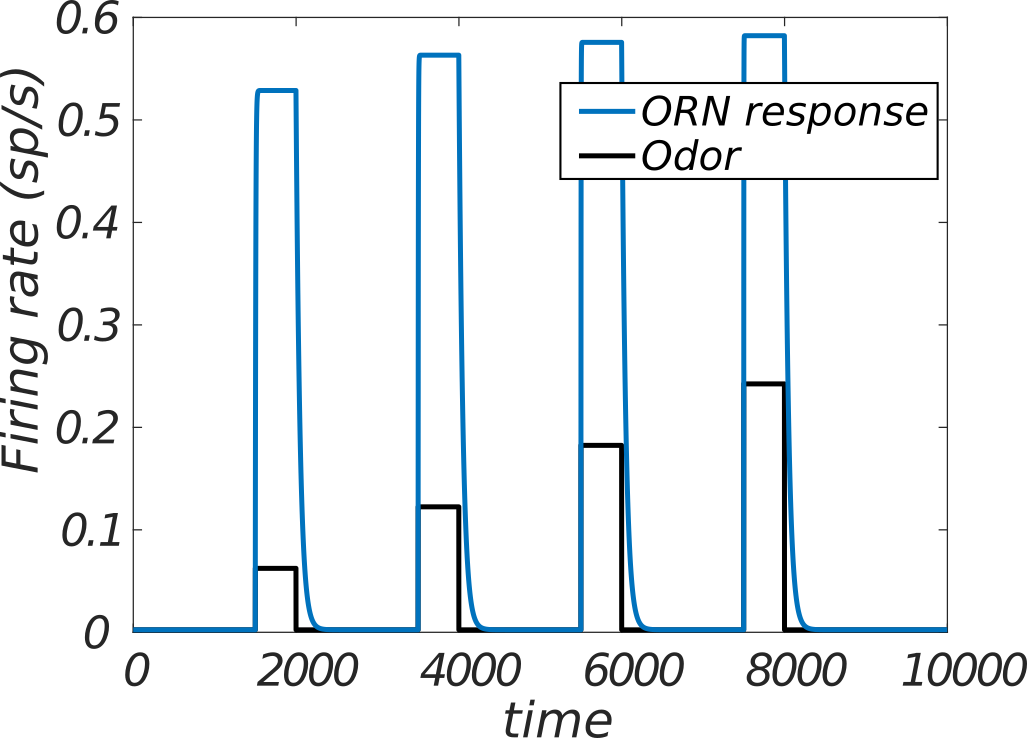
\includegraphics[scale=1]{2016-08-05DynORNnoInactivation.png}
\label{fig:orn3}
\end{figure}
Unsatisfied with the shape of the ORN response in this model, we began to experiment with various inactivation terms.  We first used a paradigm in which bound receptor ($R^*$) could vary between an active and inactive ($R^i$) state (data not shown).  We then converged on a model in which inactive receptor recycled back to the unbound state ($R$).  We modeled this with the following equations:
\begin{equation}
\frac{dR^*}{dt} = k_{on}[O] + (k_{re} - k_{on}[O])\,R_i - (k_{on}[O] + k_{off} + k_{de})\,R^*,
\end{equation}
\begin{equation}
\frac{dR_i}{dt} = k_{de} \,R^* - k_{re}\, R_i,
\end{equation}
where $R_i$ was the inactive state, $k_{de}$ was the constant of inactivation (from $R^*$ to $R_i$), and $k_{re}$ was the constant for the conversion from $R_i$ to $R.$  

This model (Figure \ref{fig:orn4}) kept the onset-concentration dependence, and was able to mimic the various shapes of (onset-transient response) curves seen in \cite{Nagel2011}.  These neurons were the ones used for later modelling (if future models require it, offset neurons can be generated using the linear filter model, but none were used for the LN or PN simulations discussed here).

\begin{figure}
\centering
\caption{\textbf{ORN firing rates: Dynamic model with one-way inactivation.}  Odor strength (in black, at bottom) is in arbitrary units.\newline}
\hspace*{-1cm}
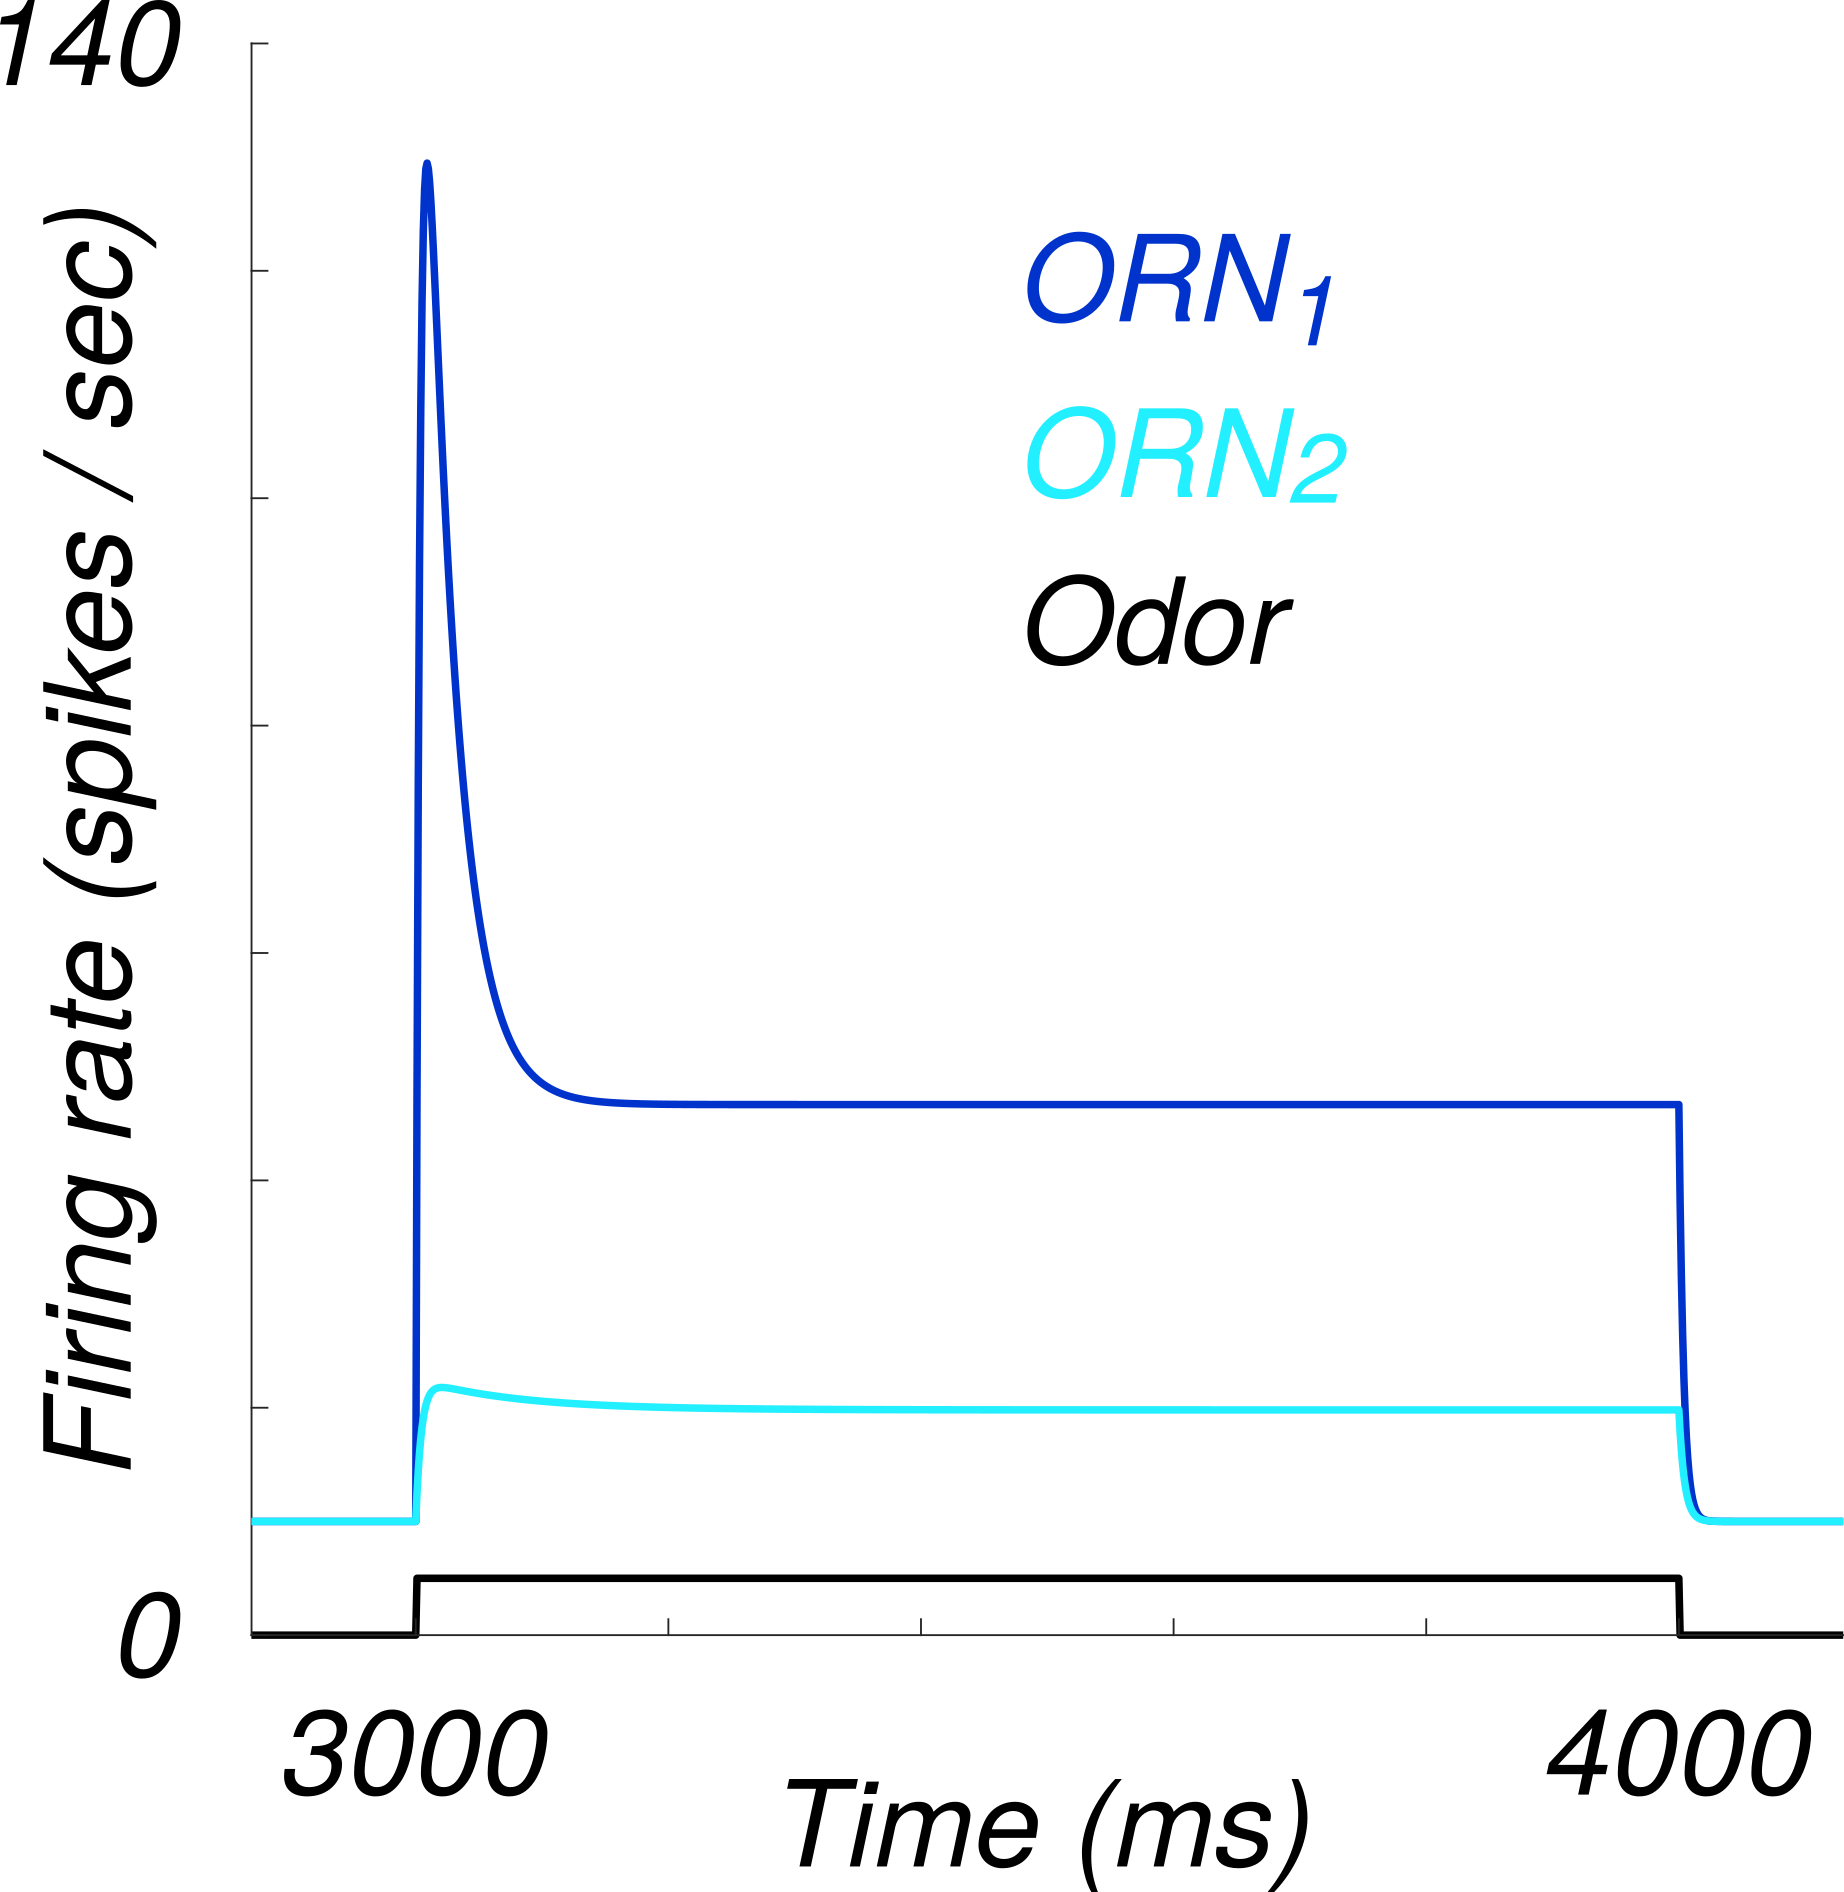
\includegraphics[scale=0.6]{2016-08-19_ORN_dynamic_responses.png}
\label{fig:orn4}
\end{figure}

\section{LN model}
To model LNs, we used a two-stage model.  The first step was to generate a series of "basis-functions", where each LN was temporally linked to the onset of odors (importantly, because odors were always simulated as idealized, consistent step functions, we used odors, not ORN responses, to trigger LN basis functions).  Each LN basis function was evenly spaced from other LNs, and together, they tiled the range of step-durations used.   Two types of basis functions were used: The first type was a set of simple delta functions (depicted in Figure \ref{fig:ln1}), where each time bin had exactly one responsive LN delta function assigned to it (leading to an unrealistically large number of simulated LNs).  The second type was a set of tightly overlapping gaussian functions (reducing the number of required LNs to a more physiologically plausible $200$ (reviewed in \cite{Nagel2016}). Gaussian peaks were spaced $6$ bins apart, and are depicted in Figures \ref{fig:ln2}.  For both types of basis set, a delay was added between odor onset and the first LN basis function.

After the basis set was generated, the second step was to project the ORN responses from all simulated ORNs on to the LN population, to mirror the all-to-all ORN to LN projections seen \textit{in vivo} (Wilson, 2004).  This projection is depicted in Equation \ref{eq:LNrate}.
\begin{equation}
\vec{r}_{LN}(t) = \sum\limits_{i} ^{N_{ORN}}{\vec{b}_{LN}(t)^T * \vec{r}_{ORN}(t)},
\label{eq:LNrate}
\end{equation}
using $\vec{r}_{LN}(t)$ as the firing rate of all LNs at time $t, \vec{b}_{LN}(t)$ as the value of the basis set (either delta functions or gaussians) at time $t,$ and $\vec{r}_{ORN}(t)$ as the firing rate of all ORNs in the system at time $t.$  This results in a vector with a length corresponding to the number of ORNs.  The firing rate was then the sum of this vector.


% One potential improvement may be to bias the LN spacing towards the onset ala Kennedy et al.
\begin{figure}
\centering
\caption{\textbf{LN basis set: Delta function with uniform delay.}  Odor strength (in black, at bottom) is in arbitrary units. Each spike corresponds to a different LN. }
\hspace*{-1.0cm}
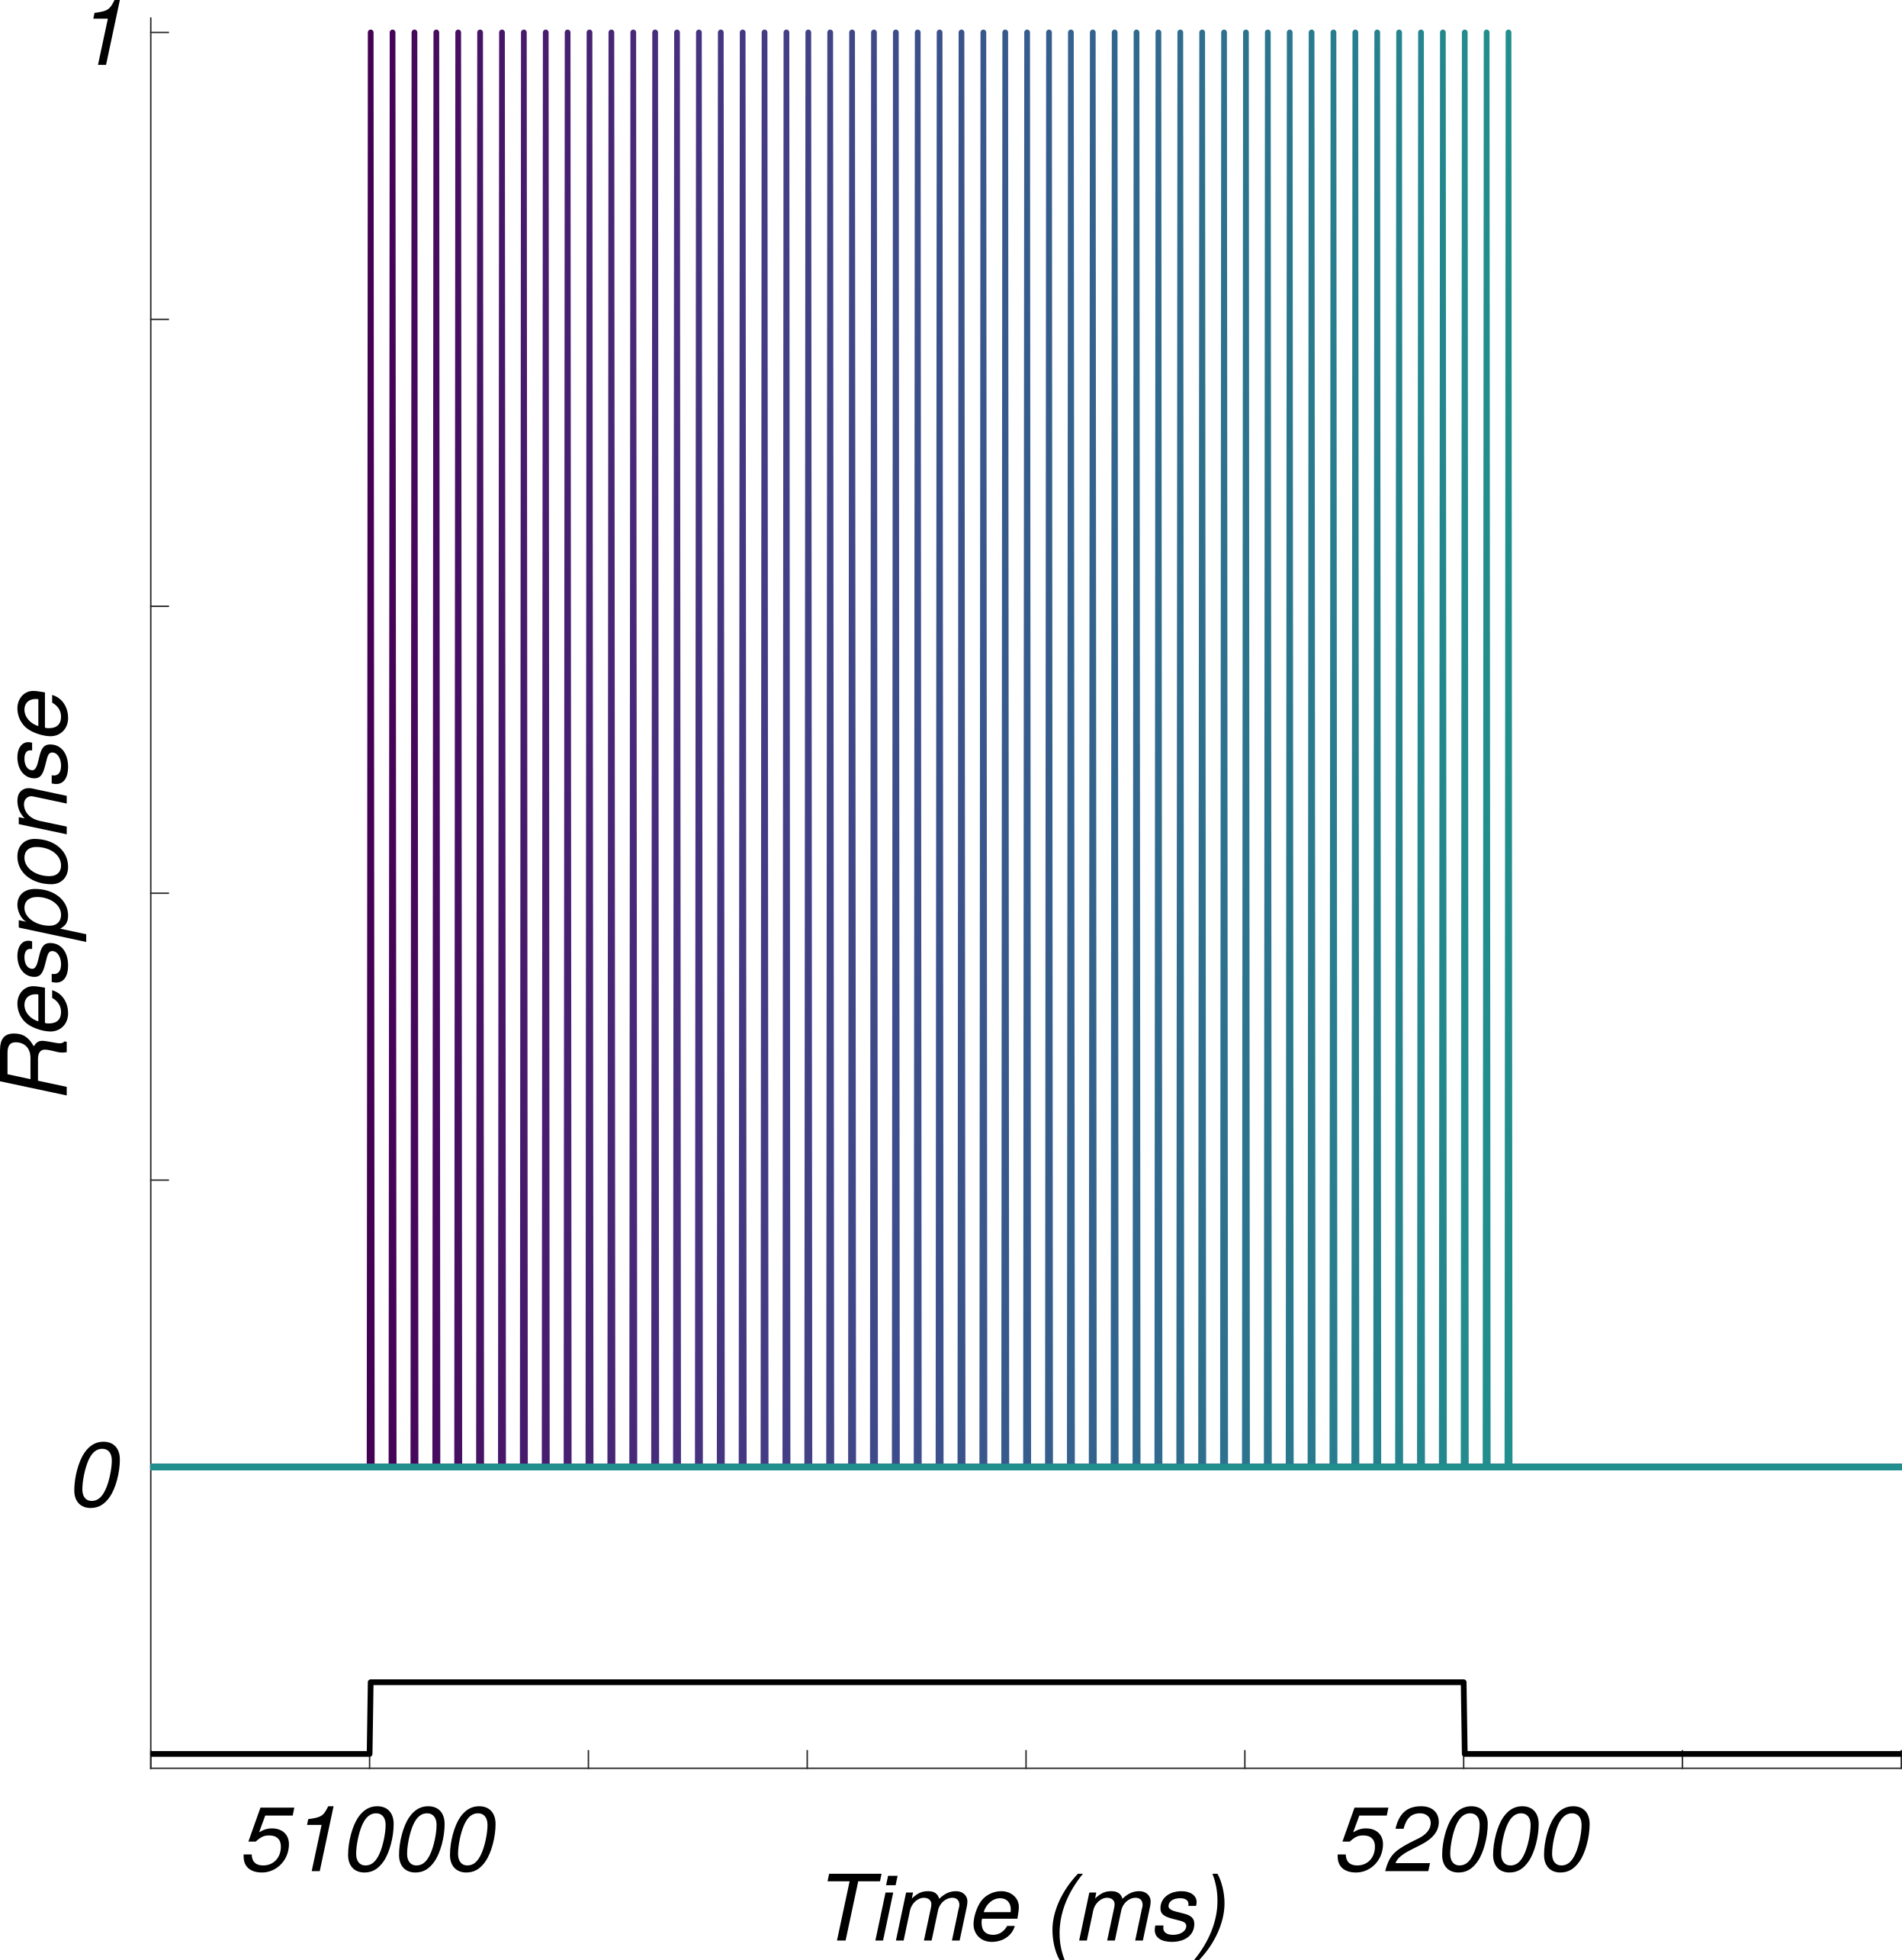
\includegraphics[scale=0.4]{2016-08-19_LNdelay_basis.png}
\label{fig:ln1}
\end{figure}
\begin{figure}
\centering
\caption{\textbf{LN basis set: Evenly spaced gaussians.}  Odor strength (in black) is in arbitrary units.}
\hspace*{-1.5cm}
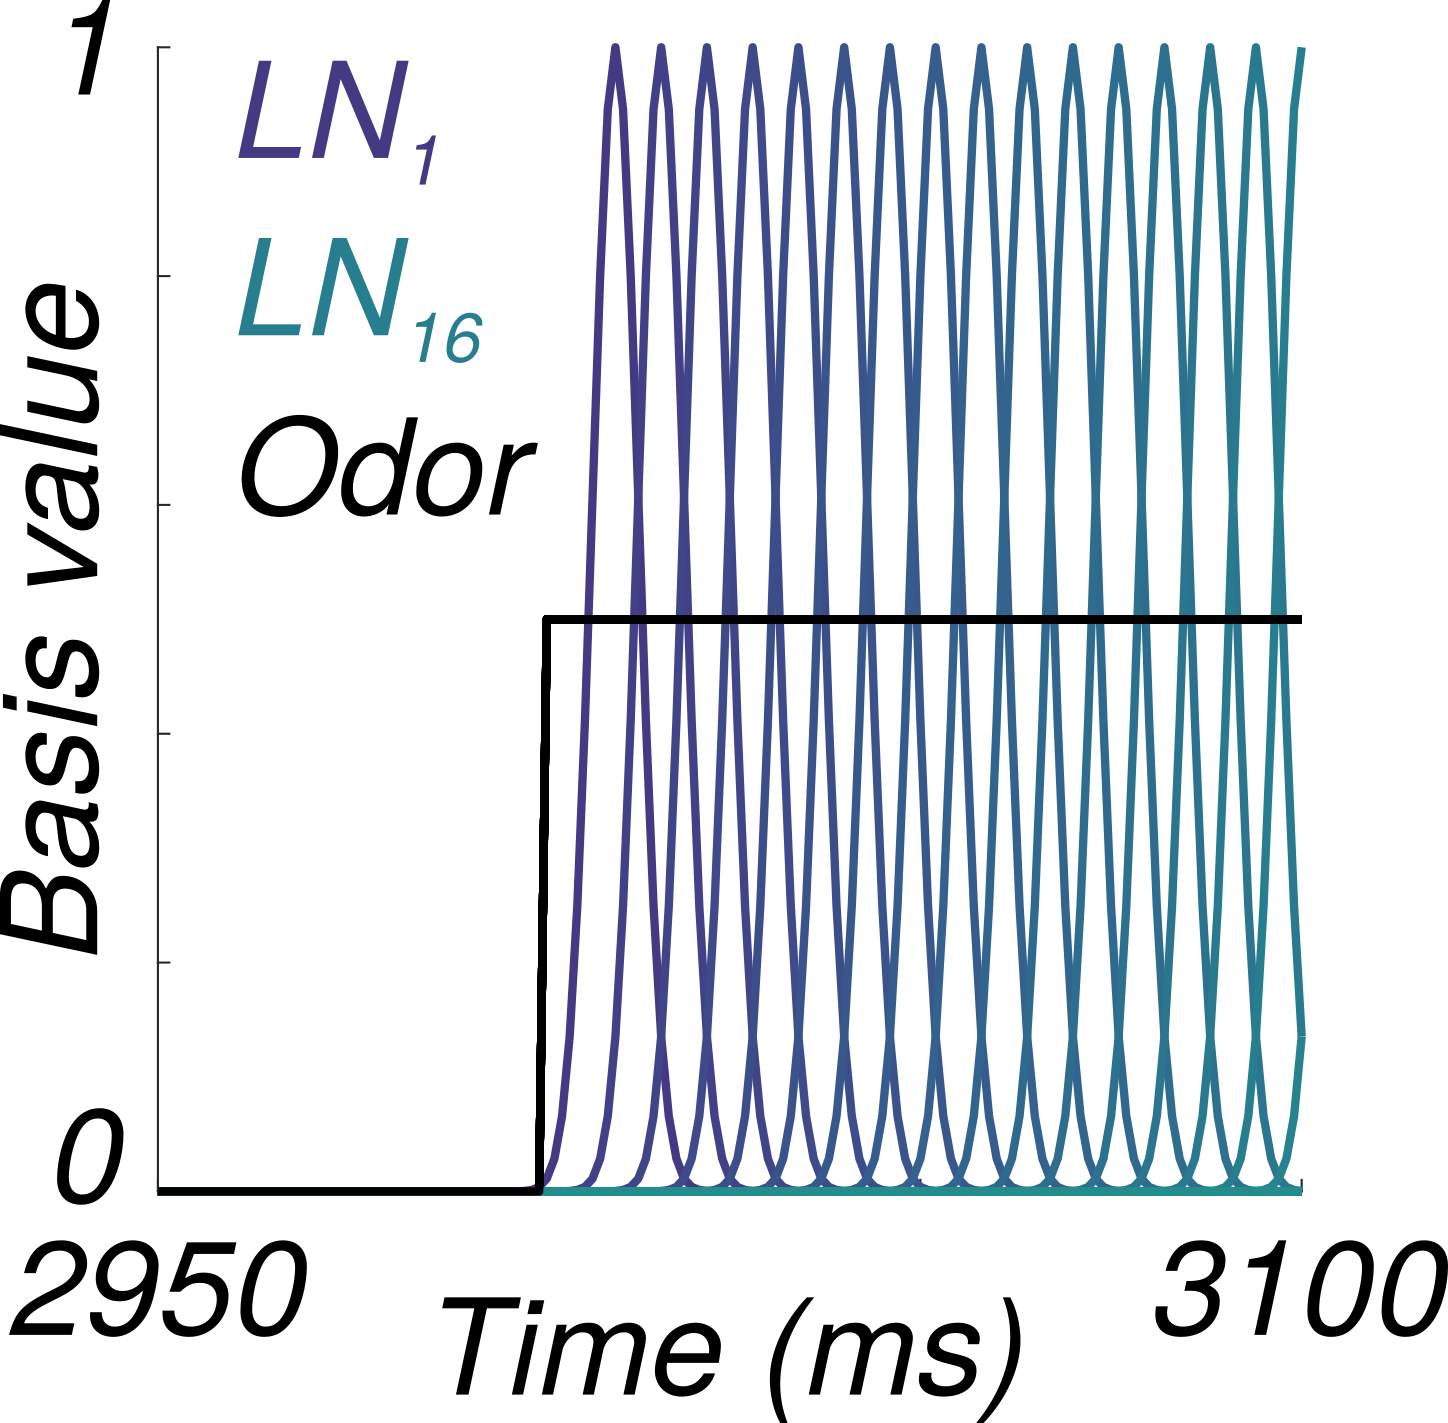
\includegraphics[scale=0.7]{2016-08-26_LNgaussianBasis_excerpt.png}
\label{fig:ln2}
\end{figure}

\section{PN model}
To test our main hypothesis, we used a simple learning rule governing the inhibition from LNs to PNs.  We modeled the inputs to PNs as a simple additive combination of ORN and LN inputs, with a PN receiving exactly one ORN input (one-to-one ORN to PN connectivity) and LN inputs from the entire population of LNs (all-to-all LN to PN connectivity).  We modelled the firing rate of a given PN $i$ as:
\begin{equation}
r_{PN_i}(t) = r_{ORN_i}(t - 1) +  \Big(\beta * \vec{r}_{LN}(t - 1)^T * \vec{w}\Big),
\label{eq:PN}
\end{equation}
where $\vec{r}_{PN_i}(t)$ was the firing rate of the $ ith$ PN at time $ t, r_{ORN_i}(t - 1)$ was the firing rate of the ith ORN at time $t - 1, \beta$ was a scale factor to weaken the degree of inhibition ($\beta$ was set to values below one: $1E-6$ was used for the delta function basis, and $1E-7$ was used for the gaussian basis).  $\vec{r}_{LN}(t - 1)$ was the vector of LN firing rates at time $t - 1,$ and $\vec{w}$ was the vector of weights, which was initialized at $-0.3,$ and was restricted to negative values (or zero).

\subsection{Learning rule (weight adjustment)}
Weight adjustments for the inputs to a given ORN were modeled with the following rule:
\begin{equation}
\frac{d\vec{w}}{dt} = \vec{w}(t) - \alpha * \vec{r}_{LN}(t) * \sum\limits_{n}^{N_{ORN}} r_{ORN_i}(t) - \bar{r}_{ORN_n}(t - \tau : t)
\end{equation}
where $\alpha$ was a constant learning rate, set to $0.1$.  The weights occupied the range from $[-\infty, 0],$ and were driven by the mean firing rate of ORNs across the preceding $\tau$ bins ($\tau$ was generally set to $200 \,ms$)- note that the mean ORN firing rate included all ORNs, and not just the one whose weights were being adjusted (also of note is that the $r_{ORN_i}(t)$ term does not change with the index $n.$  

For a given LN weight to update, two conditions must be met: The LN must be active (both basis sets used a baseline firing rate of zero), and the respective ORN must have a firing rate deviating from the average across the previous $\tau$ time bins.  If either value is zero, the weight will not change.

\section{PN results}

\begin{figure}
\centering
\caption{\textbf{PN responses, early and late - delta LN basis set}  The left panel depicts an ORN and PN response during the first odor pulse; the right column depicts the same ORN and PN after learning.  Odor strength (in black) is in arbitrary units.}
\hspace*{-1.5 cm}
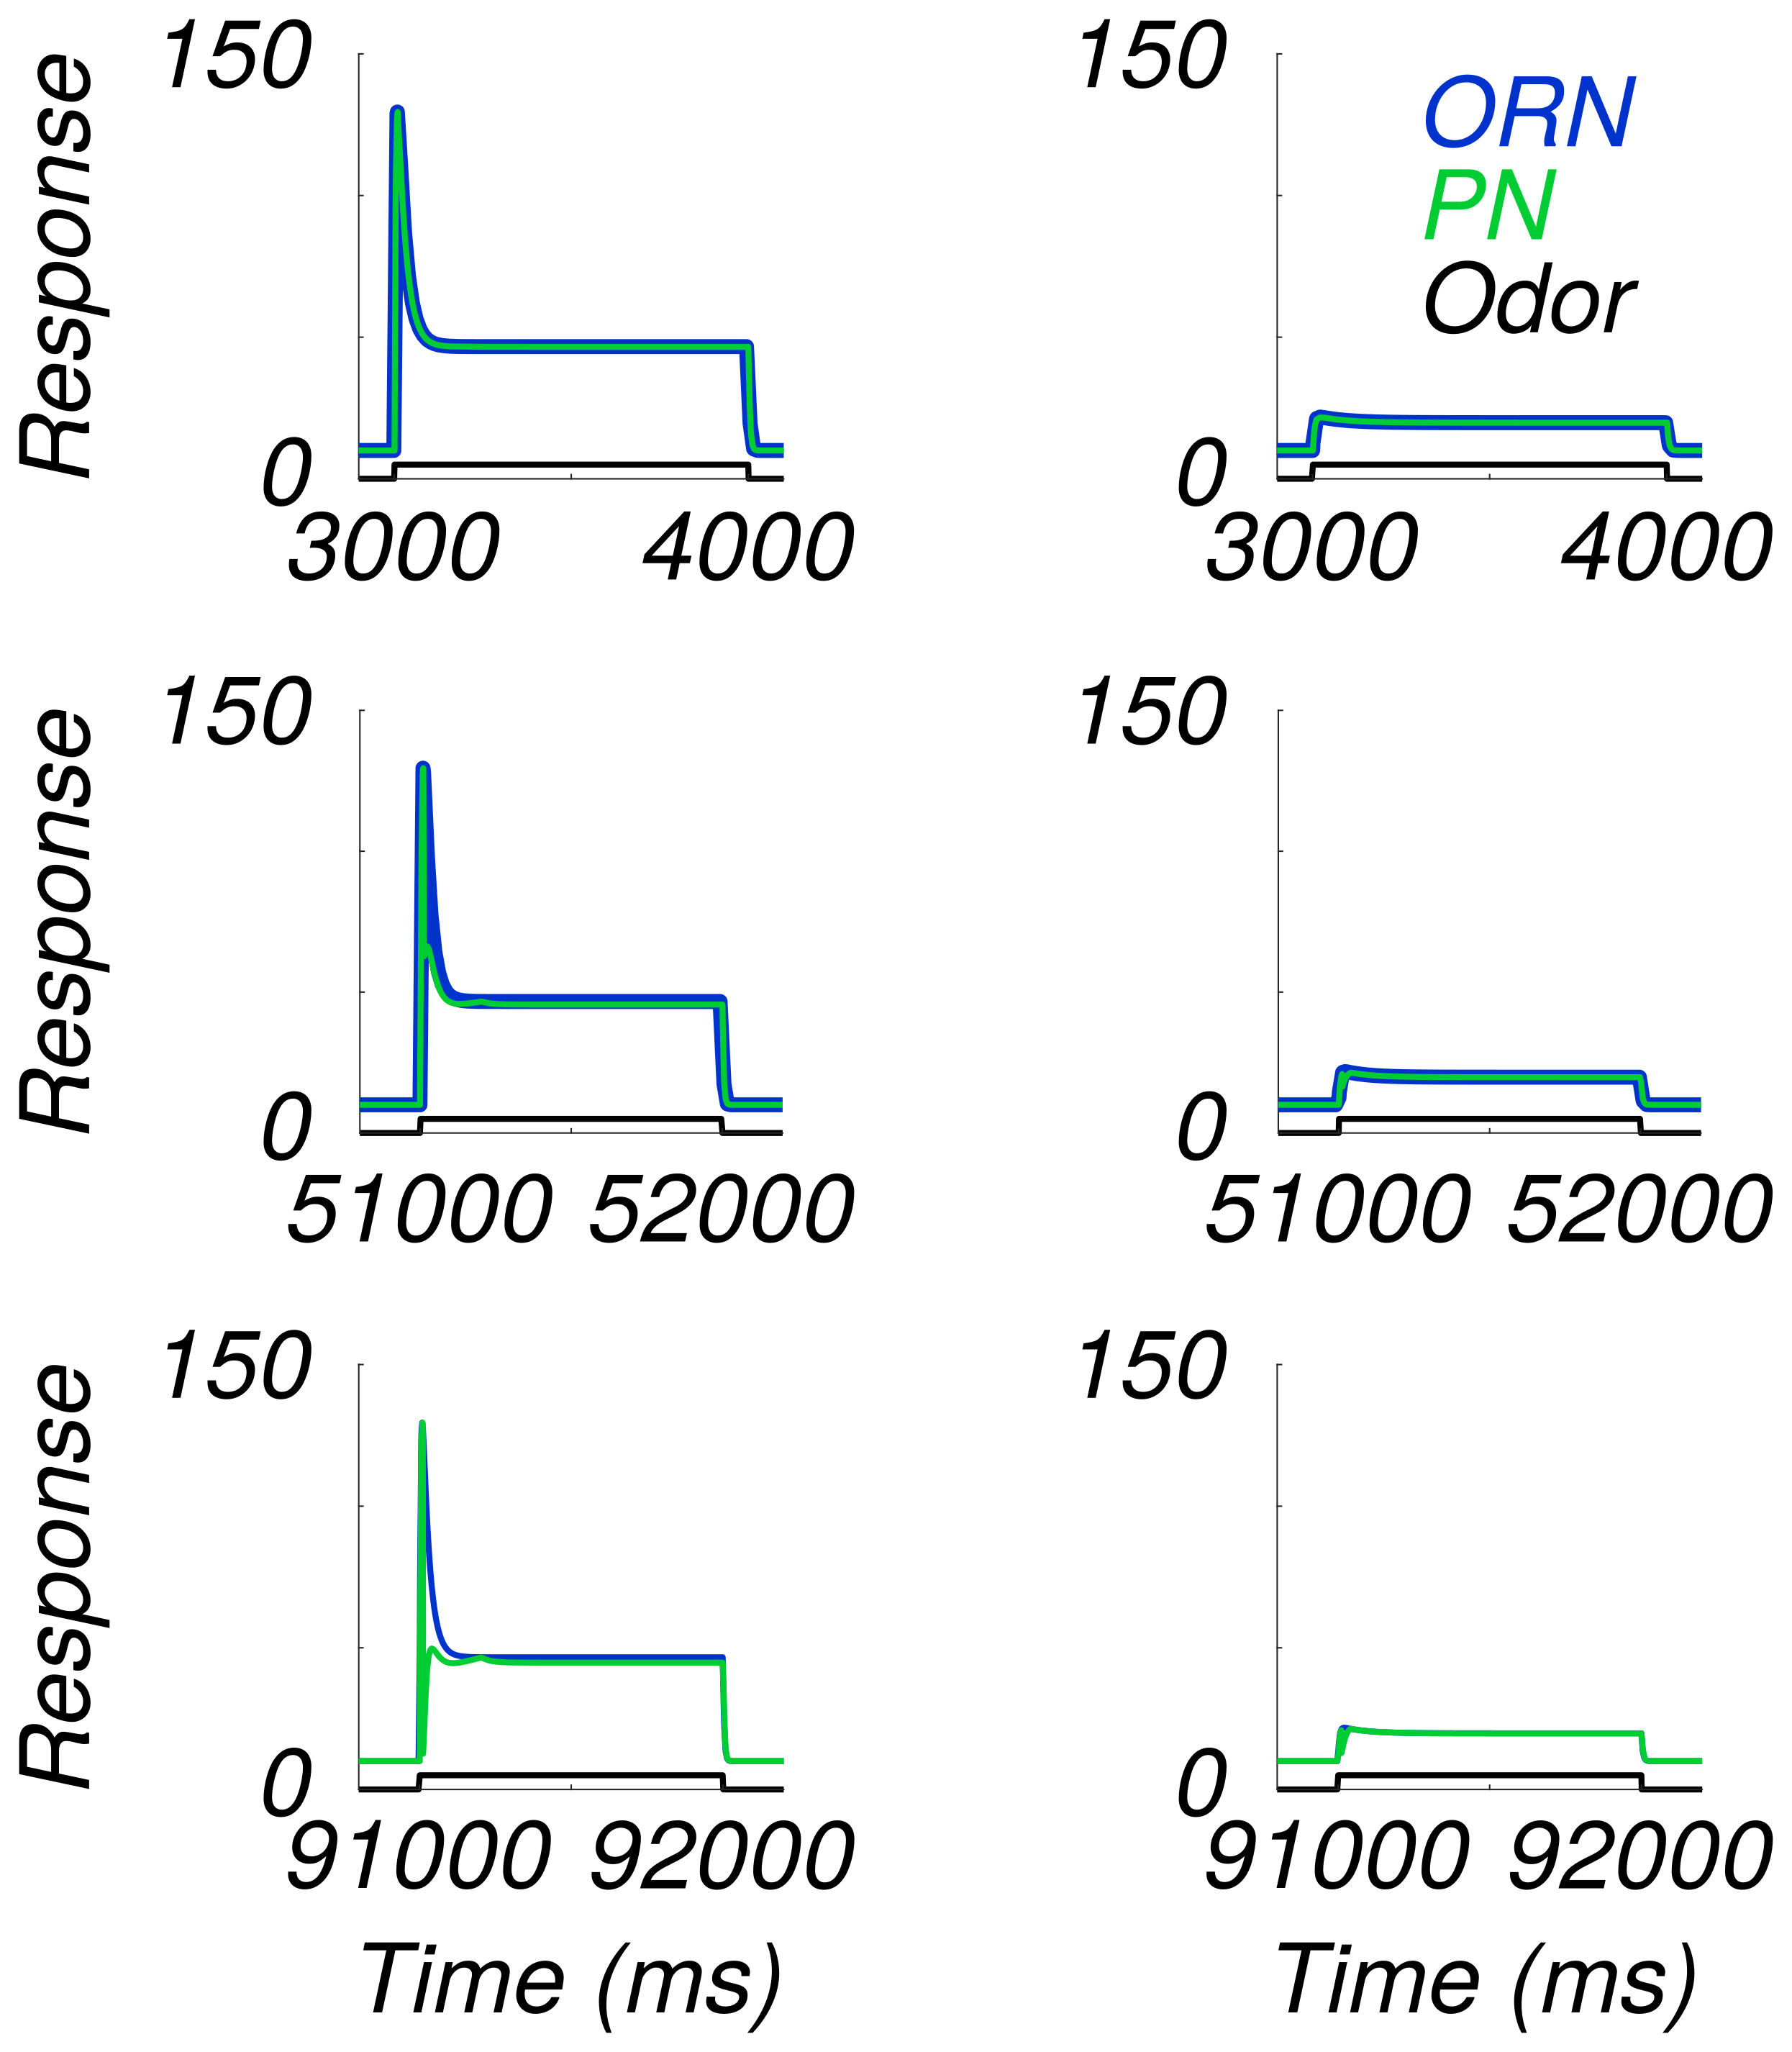
\includegraphics[scale=0.72]{2016-09-02_PN_3timepoints_deltabasis.png}
\label{fig:pn1}
\end{figure}

Two sample PNs, from a set of four, and using the delta basis set for the LN population is shown in Figure \ref{fig:pn1}.  For reference, ORN inputs are also shown.  The top row depicts the PN response at the first odor presentation.  At that time, weights have yet to change from their initial values.  As a result, the initial PN response closely reflects the dynamics of the ORN input.

The middle row shows the response to the thirteenth odor presentation, and the bottom row depicts the 23rd odor presentation (presentations to display were chosen arbitrarily).  Because of the imposed delay in the model, the initial ORN transient cannot be inhibited - LNs are not yet active for the first ten ms of the response.  Following this delay, for both the middle and bottom row, the effects of LN inhibition can be seen in the weakened onset response - the onset transient is no longer as strong as it is in the ORN inputs.  

Figure \ref{fig:pn2} depicts PN responses in the same manner as in Figure \ref{fig:pn1}, but using the gaussian basis set for the LNs. Results are qualitatively similar, with a noticeable difference being the weakening of the early onset transient - the non-zero width of the gaussians shortens the lag (the first LN gaussian is centered at the tenth ms after onset - the same as the first delta function).  

Regardless of the LN basis set used, the PN response rate fluctuates around the eventual steady state, before slowly converging to this steady state.  Before this steady state time, inhibition strength fluctuates, driven by the relation between recent ORN firing rates $r_{ORN}(t)$ and the rolling average $\bar{r}_{ORN_n}(t - \tau : t).$  

These slow fluctuations in PN firing rate end once the ORN firing rate has been relatively stable for $\tau$ time bins (ORN rates continuously decay, but the change is negligibly small).  Deviations from the mean ORN firing rate are small; hence the weights are too weak to substantially inhibit the ORN inputs.

\begin{figure}
\centering
\caption{\textbf{PN responses at three time points - gaussian LN basis set}  The left column depicts a model ORN with a strong onset transient; the right column depicts an ORN model with a weak onset transient.  Odor strength (in black) is in arbitrary units.}
\hspace*{-1.5cm}
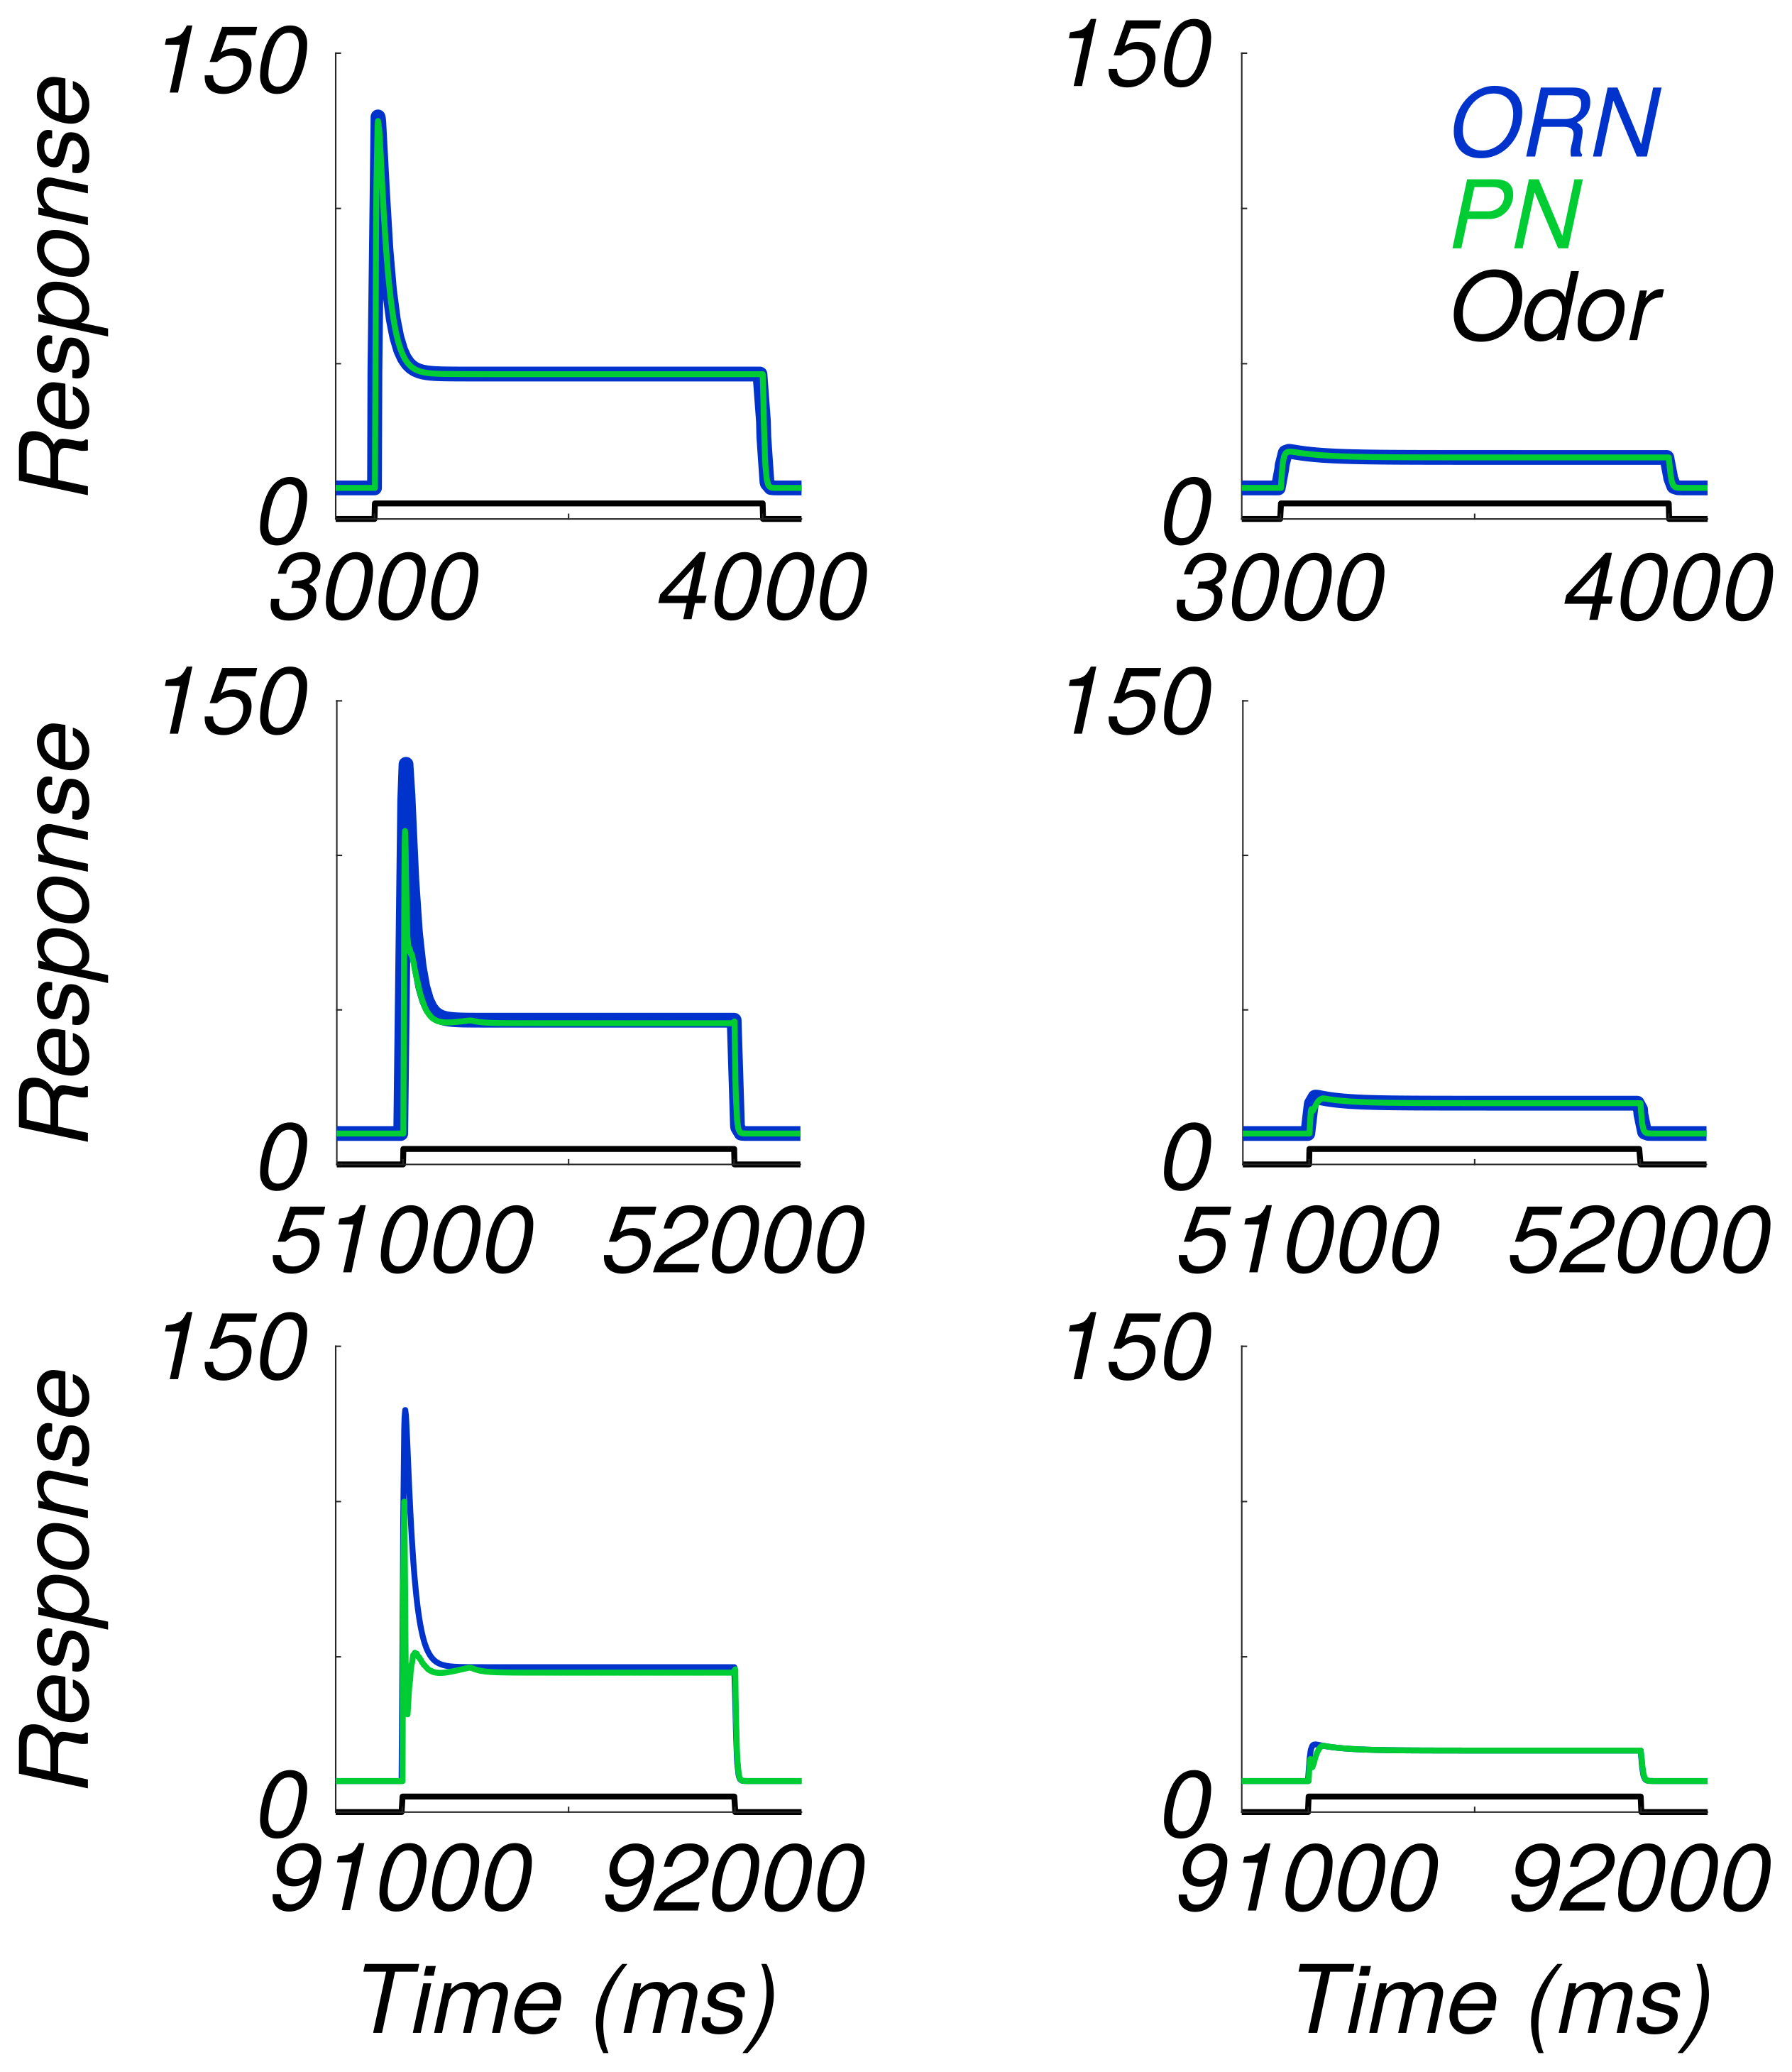
\includegraphics[scale=0.7]{2016-09-01_PN_3timepoints.png}
\label{fig:pn2}
\end{figure}

\subsection{Weights}
Figure \ref{fig:weights} shows the weights after training for both basis sets.  Because weights were unrestricted, they continue to grow for each odor presentation.  Weight adjustments are partially a function of the deviation of the input ORN firing rate (that is, from a single ORN) from the population average across the last $\tau$ ms.  Hence the early weights grow at a much higher pace than those later on.

\begin{figure}
\centering
\caption{\textbf{LN weight vectors after a 120s simulation}  The left panel depicts weights using the delta function LN basis set; the right panel depicts weights using the gaussian LN basis set.  The black trace depicts the left column of Figures \ref{fig:pn1} and \ref{fig:pn2}, while the purple trace depicts the ORN from the right column (with the weaker ORN onset transient). }
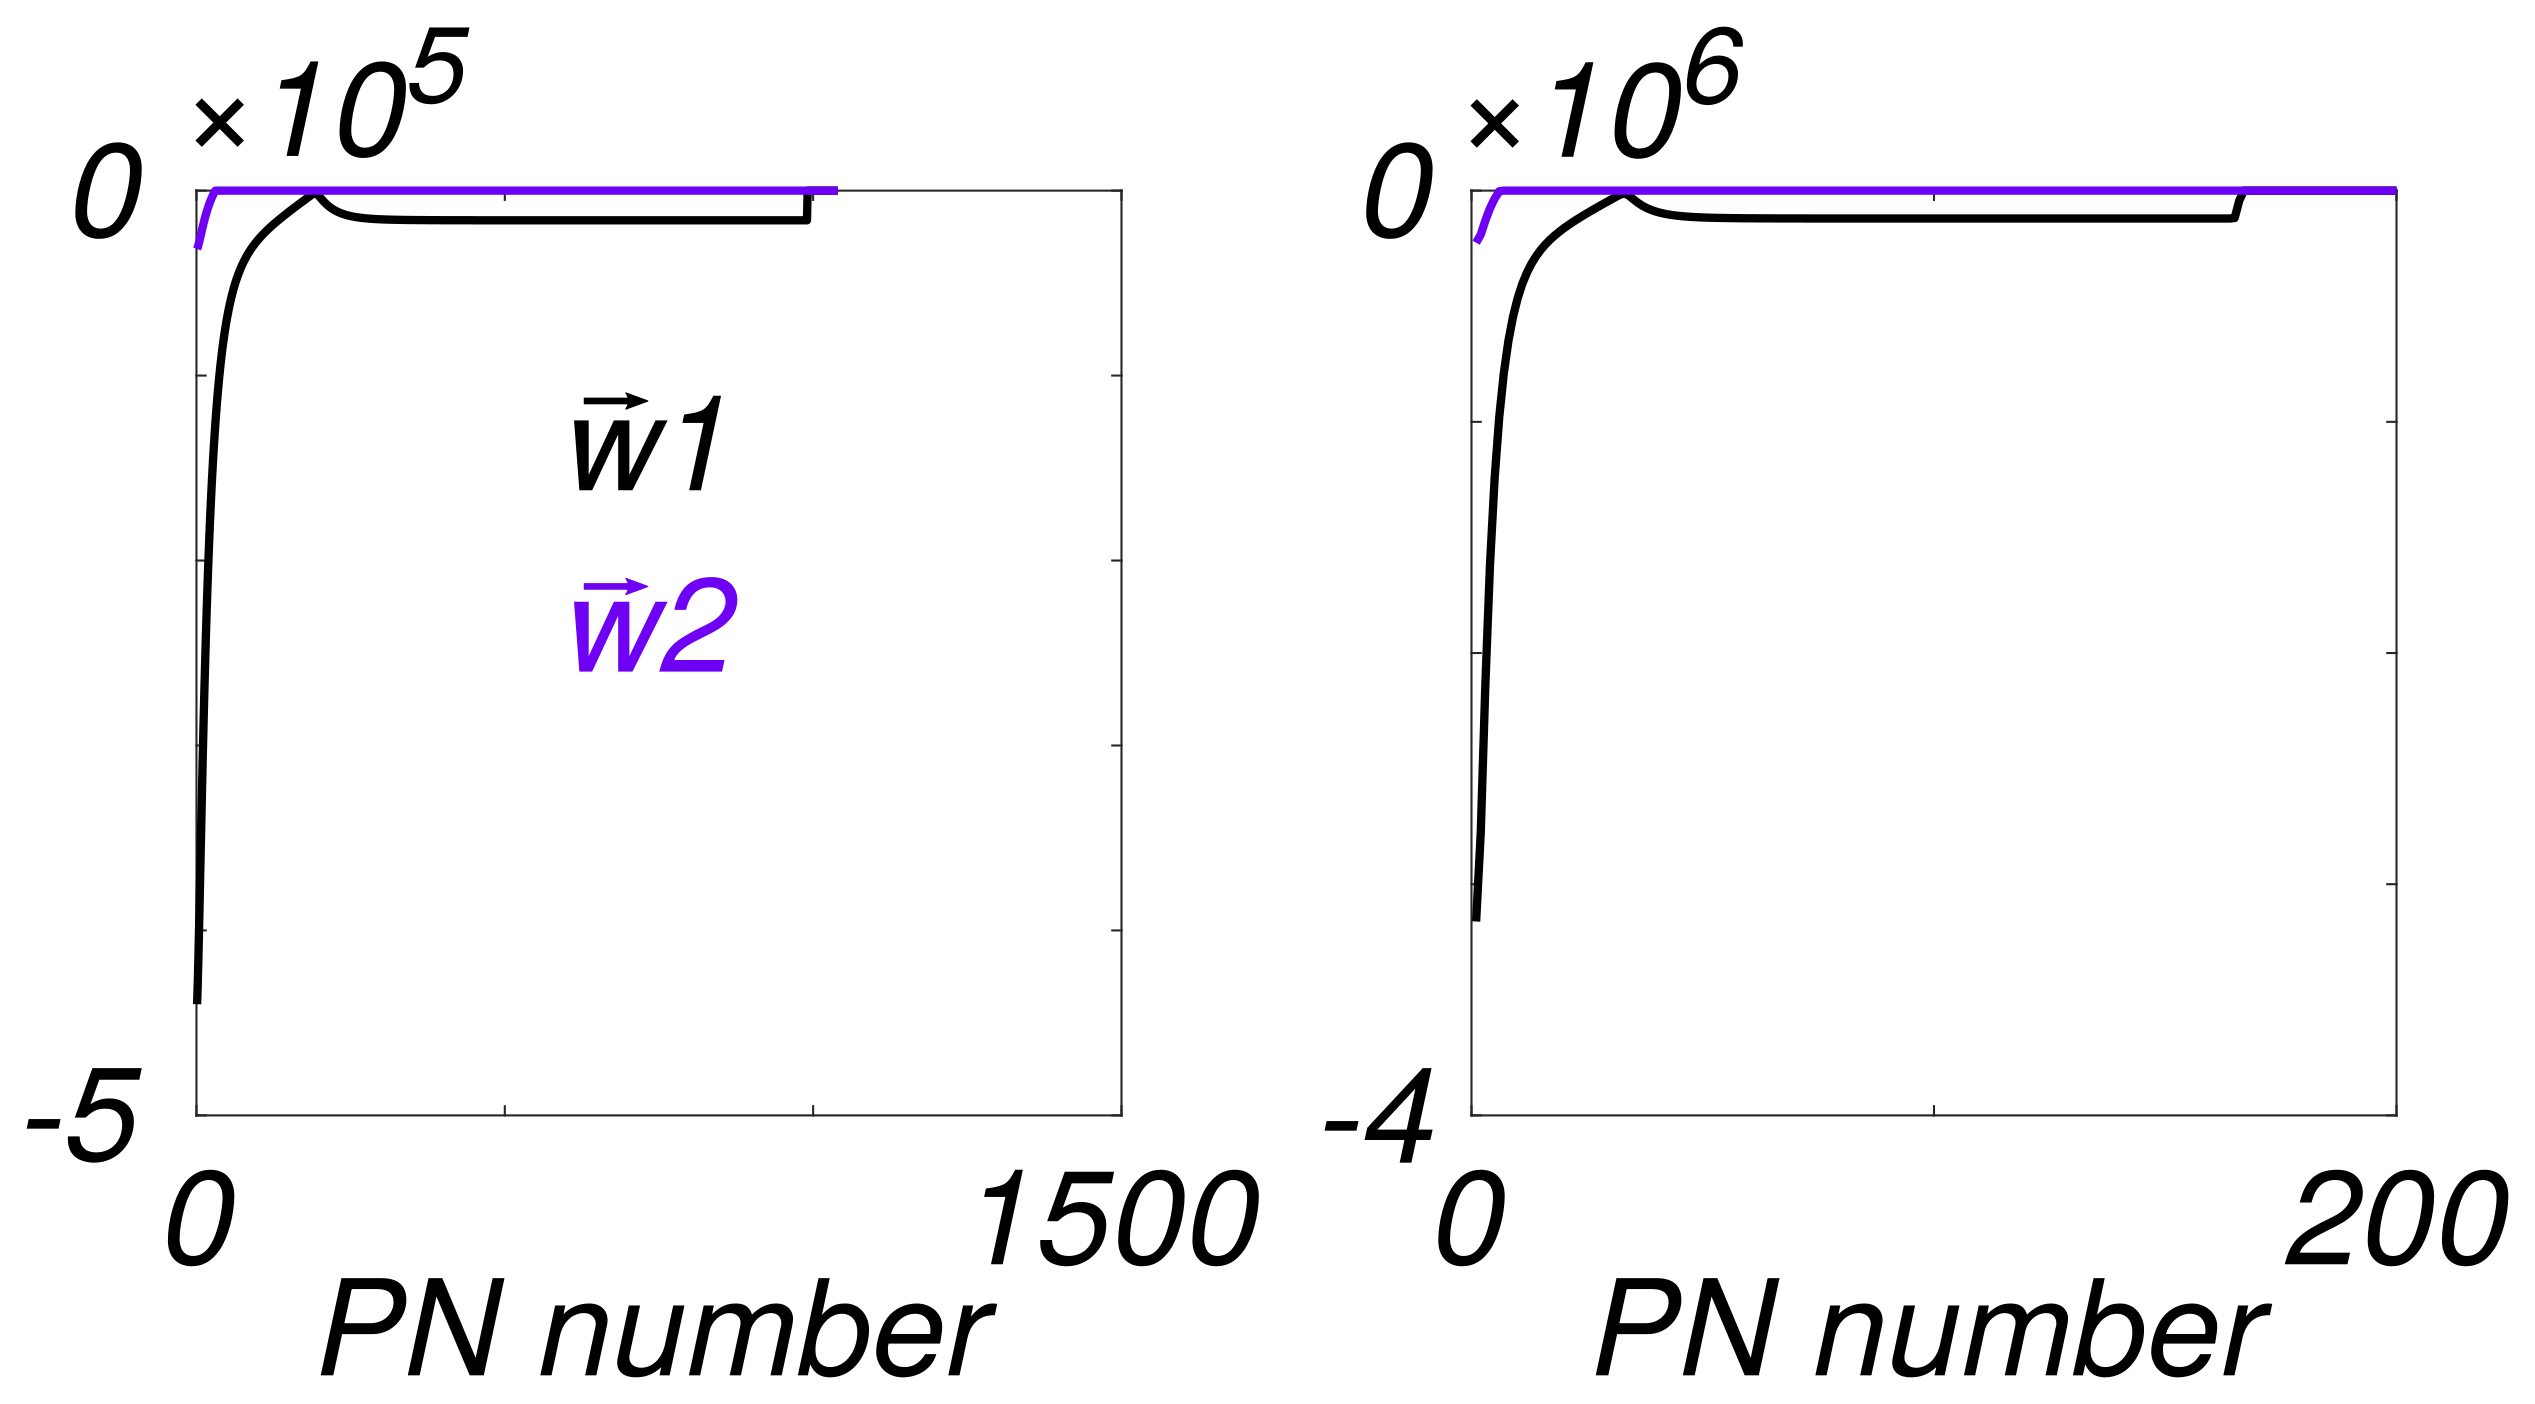
\includegraphics[scale=0.7]{2016-09-02_Delta_Gauss_weights.png}
\label{fig:weights}
\end{figure}

\section{Discussion}
We set out to investigate whether a system implementing a simple learning rule could learn to weaken onset transients, and generate a circuit output which more closely matched the original input signal.  Our model succeeded at generating a simulated PN signal that captures a number of the features seen in actual PN responses \cite{Nagel2015}, and it did so using a minimal set of parameters.  To claim that this model represents the solution used \textit{in vivo} would be a stretch (and is almost certainly untrue - weight values are extraordinarily high, and continue to grow across repeat presentations); nevertheless, it is possible that the principles driving our model - namely a Hebbian weight adjustment scheme, whereby LN inhibition learns to account for onset transients by becoming more negative - may be functionally similar to those seen in biology.  The above-mentioned example of the weakly electric fish is evidence of a similar solution to a parallel problem.  More physiological and modeling work will need to be done before any strong claims can be made; for now, it suffices to say that we have failed to disprove this model as a potential solution to the problem.

\subsection{Problems and inaccuracies}
In the creation of such a simplistic model, a number of tradeoffs had to be made.  Chief among them is the unrealistic nature of the inhibition - in our model, we had a scalar adjust inhibition to a level that was "just-right", strong enough to measurably affect the signal, while not reducing the signal to zero.  This was very much a hand-tuned quality.  The values used for $\beta$ were chosen to be in this ideal window.  A model where inhibition was either inherently balanced with the strength of excitation, or at least a physiological justification for the mechanism of inhibition would be better moving forward.  Additionally, inhibition in the ORN-PN synapse seems to be presynaptic and divisive\cite{Nagel2015}.  Our model unrealistically represented ORN-PN inhibition as both postsynaptic and subtractive.  

\FloatBarrier
\bibliographystyle{plainnat}
\def\bibfont{\footnotesize}
\bibliography{NagelRotation.bib}

\end{document}
